\documentclass[12pt, a4paper]{scrartcl}
\usepackage[utf8]{inputenc}
\usepackage{graphicx}
\usepackage{amsmath, amsthm, amssymb, textcomp}
\usepackage{setspace}
\usepackage{paralist}
\usepackage{graphicx}
\usepackage{caption}
\graphicspath{{WSK_im/}} %Graphic is in a folder named WSK_im in the currend directory
\usepackage{float}
\usepackage{authblk}
\renewcommand\Authfont{\fontsize{12}{14.4}\selectfont}
\title{Bayesian probability theory - Lesson 8:\\
Continuous probability distributions and invariance}

\author{Wolfgang von der Linden, Gerhard Dorn, Johanna Moser}
\date{Transcript}

\begin{document}
\setlength{\parindent}{0pt}
\maketitle
\onehalfspacing

Welcome to unit 8 of the course on Bayesian probability theory. My name
is Wolfgang von der Linden and I will enable you to help Captain Bayes and
her crew to deal with \textbf{continuous variables} and to learn how to\textit{assign prior probabilites}.
\begin{itemize}\item We will learn how to work with \textbf{probability densities} instead of probability mass functions.
\item We will learn how to use the \textbf{transformation law} to locate the lighthouse and the principle of \textbf{transformation invariance} will allow us to derive \textbf{Jeffrey’s prior}
\item We will study the probability distribution of the first digits of mathematical tables.
\end{itemize}


\section*{Continuous variables}
Up to this point we have actually only introduced the rules of probability
theory for \textbf{discrete variables}. But you certainly realized that \textbf{continuous
variables} have also crept into the problems of the last unit, for example in the star
path problem or the fishing ground problem. We even mentioned probability
densities. \\
The values of the parameters in the continuous case can take on
\textit{any real number} in a given interval or even on the entire real axis.
Now it’s time to extend the rules of probability theory to continuous variables.\\

Let’s start with the following consideration: Assume we are interested in the height of trees. Typically it ranges between 0 and and a maximum height $h_{max}$. To get started we discretize the possible heights into $N$ intervals of equal length. For simplicity, we assume that all heights are equally probable. Therefore,
the probability that the height $l$ of a randomly selected tree lies in
the interval $I_i$ is the same for all intervals.
\[P(\Delta I_i)=\frac 1N = \frac{\Delta l}{l_{max}}\]%

Two things are important to note here:\\
a) If we increase the number of intervals the probability goes to zero. So
the \textit{probability for a continuous variable to have a precise value is zero} and
hence it makes no sense to speak of probabilities or to use a probability mass
function to assign probabilities to certain variables.\\

\fbox{\parbox{\linewidth}{\textbf{Question 1.} Which of the following statements are true?\\
a) The height of trees shall be uniform in the interval [0,30]. Then, the probability for a tree to have a height of 20 meters is $\frac{1}{30}$.\\
b) The height of trees shall be uniform in the interval [0,30]. Then, the probability to have a tree of 15 to 17 meters is $\frac{1}{15}$.\\
c) The height of trees shall be uniform in the interval [0,30]. Then, the probability to have a tree of 14 to 16 meters is $\frac{1}{15}$.\\
d) Assuming a unifor mistribution with the probability given for an interval $P(\Delta I)=A$, the probability for $P(\Delta I/2)=A/2$.
}}
\\

b) We see that the probability is \textit{proportional to the interval size} $\Delta l$ .\\
Both points stay valid in the case of non-equidistant intervals and also if the height
distribution of trees is not uniform.\\

In general, we find for the probability, that the height of a tree lies in a certain interval, is \textit{proportional} to the length of this interval. The proportionality function is the \textbf{probability density} $p(l)$.
 It is the probability to find a tree with a length in the interval $[l,l+\Delta l]$ divided by the interval length.
 \begin{equation*}\boxed{p(l)=\frac{P(\Delta I_l)}{\Delta l}
}\end{equation*}\\
The probability for the height of a tree to fall into an interval can also be obtained
form the difference
\[P(\Delta I_l)=P(\text{height}\leq l+\Delta l)-P(\text{height} \leq l)\]

We introduce a special function $P(\text{height}\leq l)=F(l)$ for these probabilities, which are called \textbf{cumulative distribution functions}. %
The reason for this term becomes clear when we rewrite $p(l)$ in
terms of the cdf:\\
\[p(l)=\frac{F(l+\Delta l)-F(l)}{\Delta l}\]

For infinitesimal interval length the pdf turns into the \textit{derivative} of the cdf
and in turn the cdf is the integral of the pdf.\\
 \begin{equation*}\boxed{F(l)=\int_0^lp(l')\text{d}l'
 }\end{equation*}\\

That explains why it is called cumulative. We also see that the normalization
implies that the cdf approaches 1 when the length approaches the upper
limit of the the range of this random variable.\\

\fbox{\parbox{\linewidth}{\textbf{Question 2.} Which of the following statements are true?\\
a) If the pdf is Gaussian, then the cdf is also Gaussian.\\
b) If the pmf is given, then the pdf can be obtained by the derivative.\\
c) If I want to know the probability that a tree is at max 20 meters high, I can use the cdf $F(20)$.\\
d) The cdf has the following form: $F(x)\propto x^2$. Then the pdf reads $p(x)\propto x$.
}}
\\

To keep the notation clear, we denote pdfs with the lowercase letter $p$ and
stick with the uppercase letter $P$ for the probability mass functions.\\

\section*{Calculations with continuous variables}
The sum and product rule are the same for continuous and discrete variables.
But the normalization and the marginalization rule are slightly different, as we do have integrals instead of sums. %8_1
 \begin{figure}[H]
	\centering
	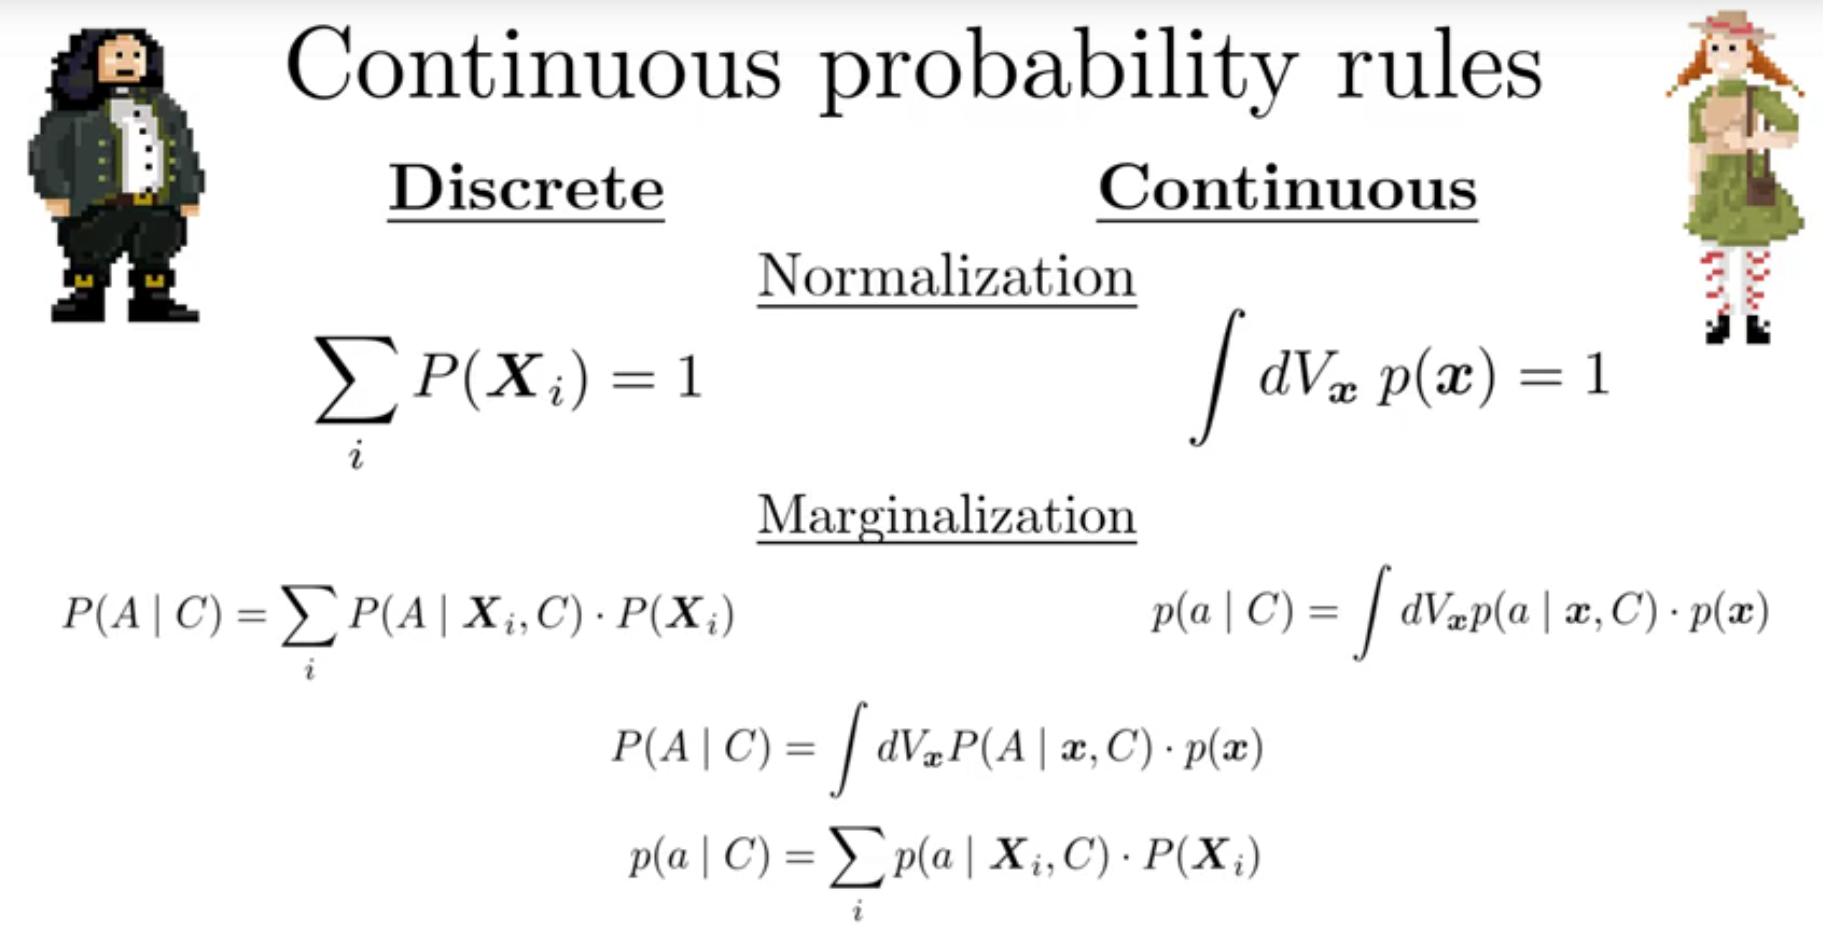
\includegraphics[width=0.75\textwidth]{8_1.png}
\end{figure}
Here, the difference between the four marginalization formulas is that capital letters stand for discrete lower case letters for continuous variables. Similarly, the mean value of functions $f(x)$ of continuous random variables x are also converted to integrals. \\
\begin{equation*}\boxed{\langle f(X)\rangle = \sum_i f(X_i)P(X_i)\qquad \langle f(x)\rangle = \int \text{d}x f(x)p(x)
}\end{equation*}\\
Here, the probability mass function is replaced by the pdf.\\


Now there is a specialty of continuous variables: You can introduce \textbf{transformations} like $l\mapsto m(l)=l^3$, which for a spherical tree would be proportional
to the mass and if one is interested in the mass then the corresponding pdf would be $p(m)$. Then a question occurs naturally: \textit{If we know the pdf $p(l)$ for the length what is the pdf $p(m)$ for the mass?}\\

The probability, that the height of a tree lies in the interval $[l,l+\Delta l]$, is given by d$P$.
The mass of these trees lies in the interval $[m,m+\Delta m]$. Since they are the same trees, we can express dP in terms of the mass and finally, due to the unique relation ``$m$ is a unique function of $l$ and $l$ is a unique function of $m$'' (i.e. bijection), we obtain the very important transformation law.\\
\begin{equation*}\boxed{p(m)=p(l(m))\left|\frac{\text{d}l(m)}{\text{d}m}\right|
}\end{equation*}\\

For the case of the uniform height distribution from above, $p(l)$ is constant, we
obtain the pdf for the mass. \[p(m)=\frac{1}{l_{\text{max}}}\frac{\text{d}(m^{1/3})}{\text{d}m}=\frac{1}{3l_{\text{max}}}m^{-2/3}\]

\fbox{\parbox{\linewidth}{\textbf{Question 3.} Which of the following transformations are correct?\\
a) $p(x)=\frac 1x$ and $y(x)=\frac 1x$. Then, the pdf of $y$ is $p(y)=\frac{1}{y^3}$\\
b) $p(x)=\frac 1x$ and $y(x)=\frac 1x$. Then, the pdf of $y$ is $p(y)=\frac{1}{y^2}$\\
c) $p(x)=x^2$ and $y(x)=\tan(x)$. Then, the pdf of $y$ is $p(y)=\arctan(y)^2\frac{1}{1+y^2}$
}}
\\

%8_2
 \begin{figure}[H]
	\centering
	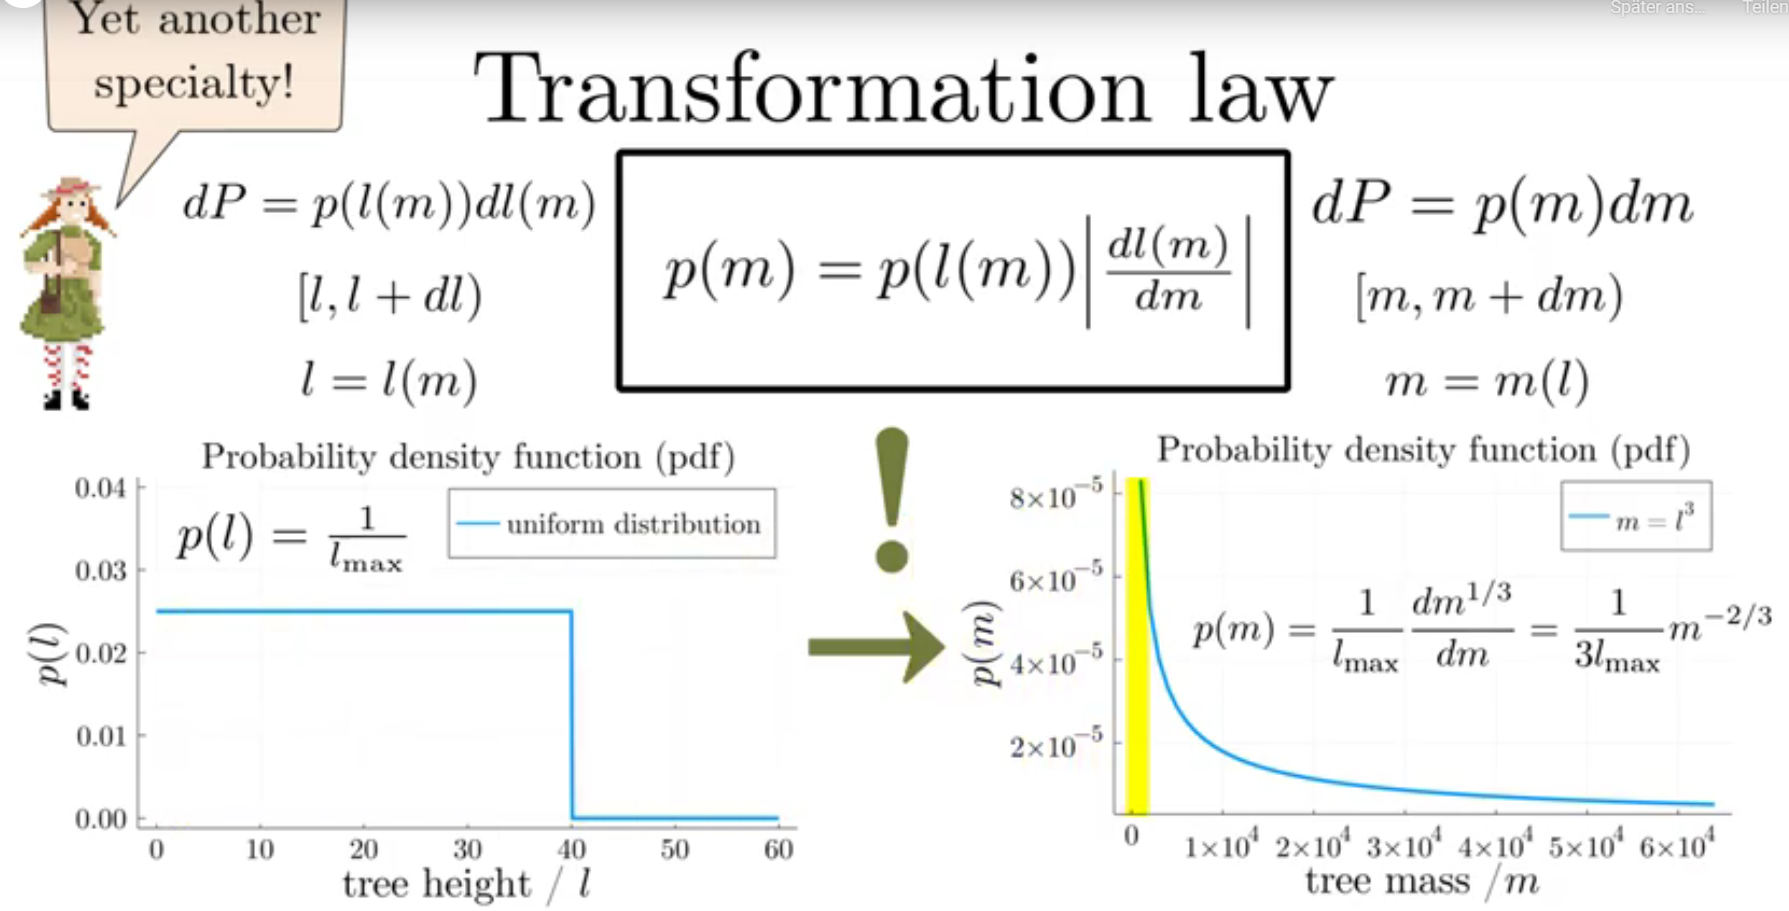
\includegraphics[width=0.75\textwidth]{8_2.png}
\end{figure}
So instead of being uniform, the pdf for the mass is sharply peaked at zero.
That brings us to a very fundamental question: \textit{How do we describe ignorant pdfs?}\\

In the discrete case the law of indifference implied equal probability but in the
case of continuous variables ignorance does not necessarily imply a uniform pdf.
As a further example, let us consider a non-negative quantity $x$ that is known
to have a uniform pdf in the interval $[0,x_{\text{max}}]$. But we are interested in the
pdf of a variable $y=\exp(x)$. The desired pdf is proportional
to $\frac{1}{y}$. So we have found, if a variable is \textit{linear on a logarithmic scale $\log(y)=kx+d$}, 
then it's pdf has a \textit{$\frac 1y$ dependance on the linear scale}.\\

Finally, we want to consider the transformation law for the \textbf{multivariate case}.
Let $\vec{x}$ be a set of variables with $N$ elements and $\vec{y}$ a new set of variables with the invertible transformations: 
$\vec{y}(\vec{x})$ is a unique function of $\vec{x}$ and $\vec{x}(\vec{y})$ in turn is a unique function of $\vec{y}$. Then the pdfs are related by the following expression, where the last factor is the \textbf{Jacobi-determinant}.\\
\begin{equation*}\boxed{p(\vec{y})=p(\vec{x}(\vec{y}))\left|\frac{\text{d}x_i}{\text{d}y_j}\right|
}\end{equation*}\\

\fbox{\parbox{\linewidth}{\textbf{Question 4.} We look at the polar transformation of a uniform pdf:\\
Given is a uniform pdf of $\vec{x}=(x_1,x_2), \vec{y}=(r,\phi)$ with $x_1=r\cos(\phi),x_2=r\sin(\phi)$. Which of the following statements are true?\\
a) The pdf of $\vec{y}$ is given by $p(r,\phi)\propto r$\\
b) If $p(\vec{x})=p(x_1,x_2)\propto x_1+x_2$, then $p(\vec{y})=p(r,\phi)=r^2(\cos(\phi)+\sin(\phi))$\\
c) The determinant of the Jacobi Matrix is given by $r^2(\sin^2(\phi)+\cos^2(\phi)=r^2$\\
d) The Jacobi matrix is given by $\left( {\begin{array}{cc}
   \cos(\phi) & -r\sin(\phi)\\
   \sin(\phi) & r\cos(\phi) \\
  \end{array} } \right)$
}}
\\

\section*{Bertrand paradox - ignorant priors}
The crew of Captain Bayes was pondering about the so-called \textbf{Bertrand paradox} which is defined as follows:\\
\textit{Given a circle of radius R and a random set of lines that cross the circle,
what is the probability that a random line has a distance from the center that is less than half the radius?}\\%8_3
 \begin{figure}[H]
	\centering
	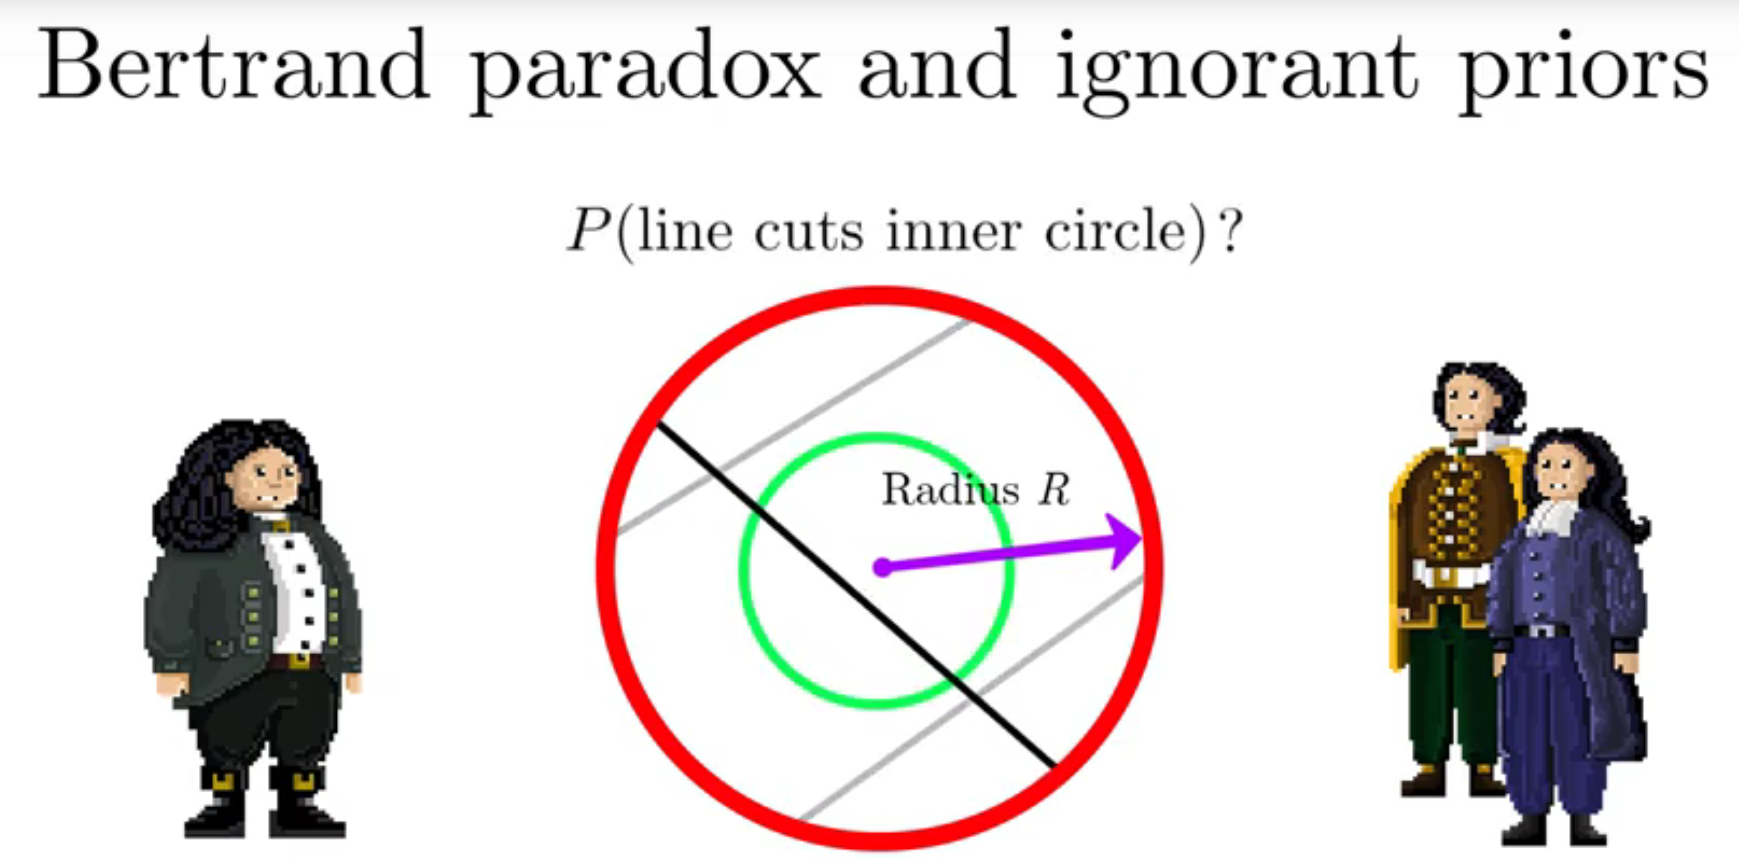
\includegraphics[width=0.75\textwidth]{8_3.png}
\end{figure}

The line cuts the circle at two points $P_1$ and $P_2$.
We can define these endpoints by the angles $\varphi_1$ and $\varphi_2$ formed by the \textit{radial lines to the endpoints with the x-axis}. These are two independent variables that uniquely define the line.\\%8_4
 \begin{figure}[H]
	\centering
	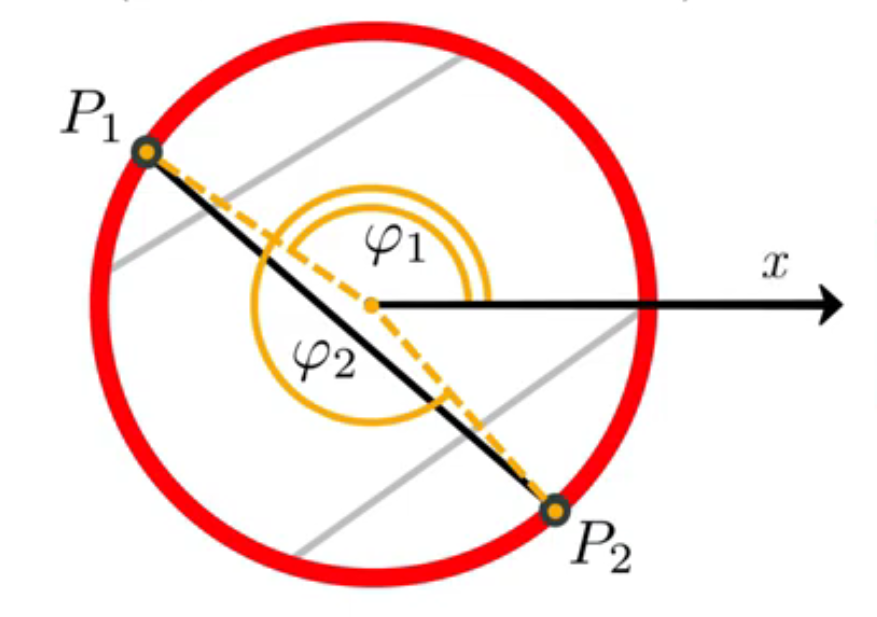
\includegraphics[width=0.4\textwidth]{8_4.png}
\end{figure}

The line is also uniquely defined by the midpoint $P$ of the two endpoints $P_1$ and $P_2$. 
This involves again two
independent variables, namely the $x$ and $y$ coordinate of the point. Finally, for solving the problem, it is enough to know the distance $r$ of the line from the center of the circle. \\%8_5
 \begin{figure}[H]
	\centering
	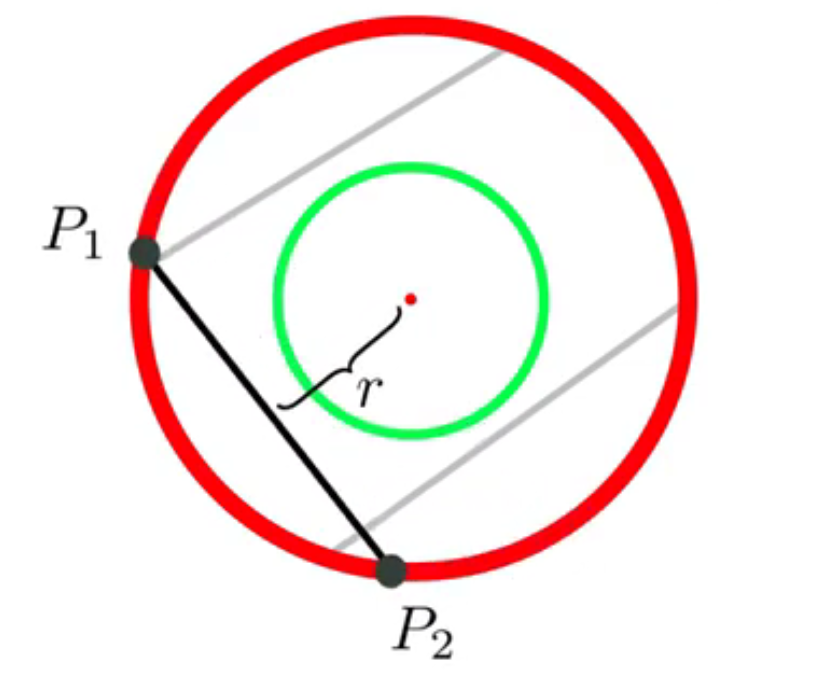
\includegraphics[width=0.4\textwidth]{8_5.png}
\end{figure}

Now think of how you would simulate the problem on the computer.
Bernoulli came up with the idea to choose the points $P_1$ and $P_2$ at random
on the circle. That is equivalent to choosing the two angles $\varphi_1$ and $\varphi_2$
at random. That in turn implies that the \textit{pdf of the intermediate angle is
uniform.}\\

In this variable, the distance of the line to the center is given by $R\cos(\varphi/2)$
 and the
condition, that the line has a distance less than $R$ half from the center, is given by \[R\cos(\varphi/2)\leq R/2\]

\fbox{\parbox{\linewidth}{\textbf{Question 5.} What is the range of $\varphi\in(0,\pi]$ fulfilling the inequality $R\cos(\varphi/2)\leq R/2$?\\
a) $\varphi \in [\pi/4,\pi/3]$\\
b) $\varphi \in [0,\pi/2]$\\
c) $\varphi \in [0,2\pi/3]$\\
d) $\varphi \in [2\pi/3,\pi]$\\
}}
\\

which implies $\varphi < \frac{\pi}{6}$. Hence the desired probability is $\frac 13$.\\%8_6
 \begin{figure}[H]
	\centering
	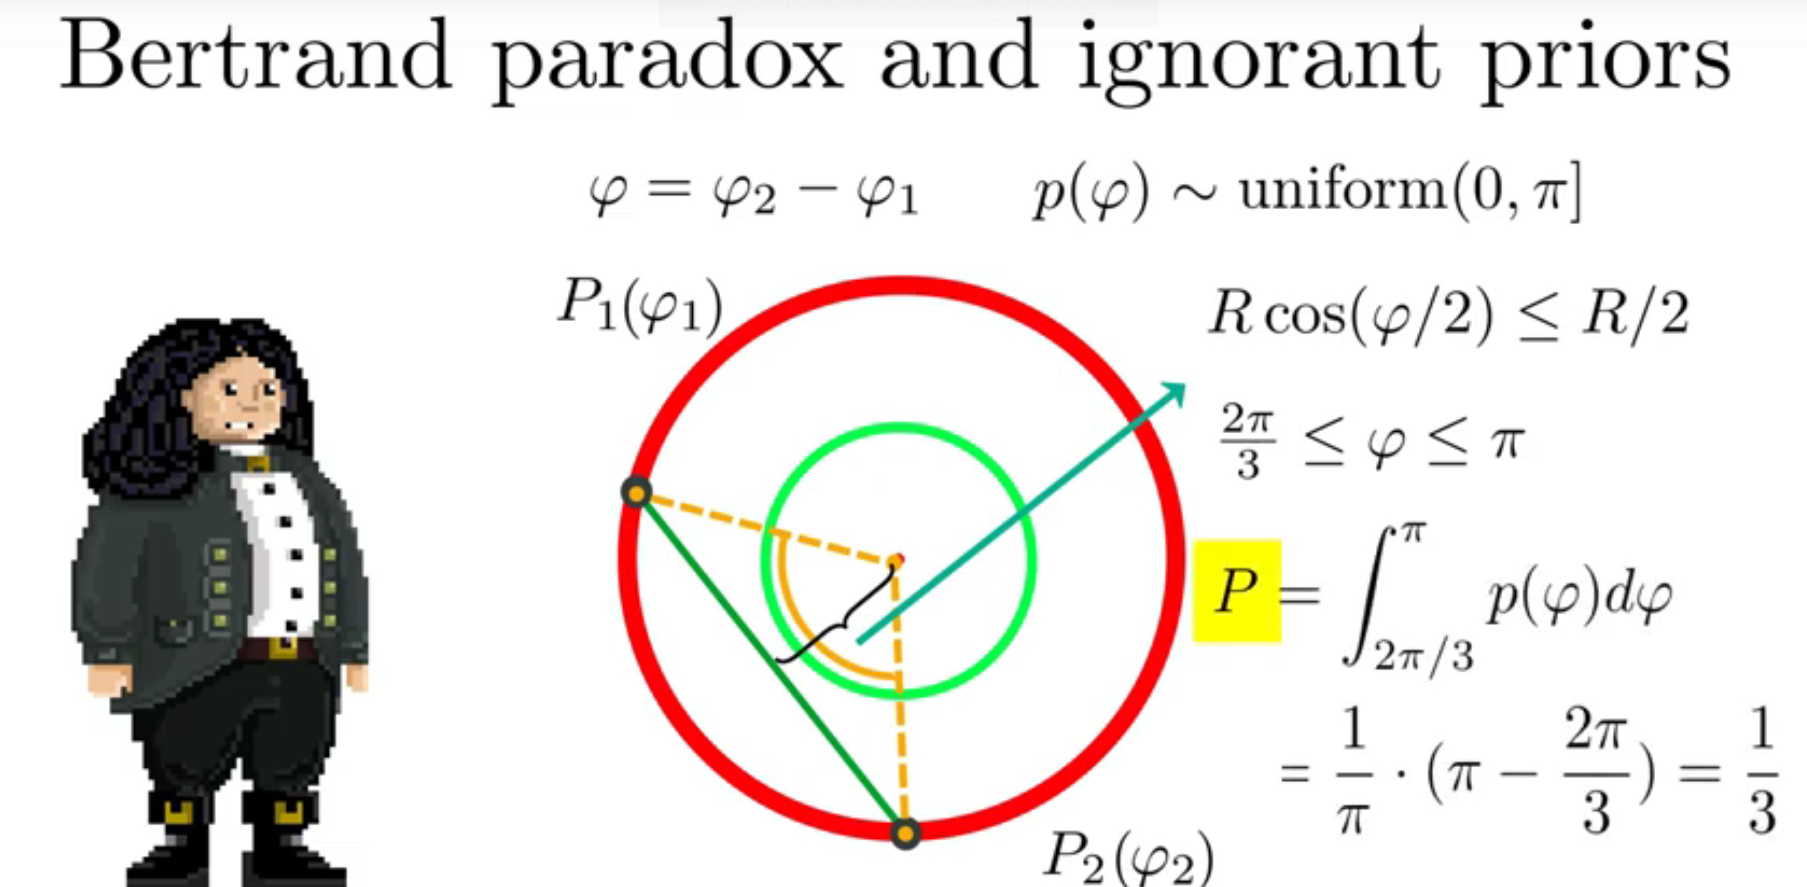
\includegraphics[width=0.75\textwidth]{8_6.png}
\end{figure}

Another way of generating the line at random was proposed in the adventure
by Pascal. She generates the midpoint at random, which means the points
are \textit{uniformly distributed within the circle}. Then the desired probability is
the probability that the point lands in the circle of radius $\frac R2$. This is a nice
illustration of the transformation law for two variables.\\
Instead of the Cartesian coordinates $x$ and $y$ we use spherical coordinates $r$ and $\varphi$. The transformation law yields for the correctly normalized pdf the following expression. %8_7
 \begin{figure}[H]
	\centering
	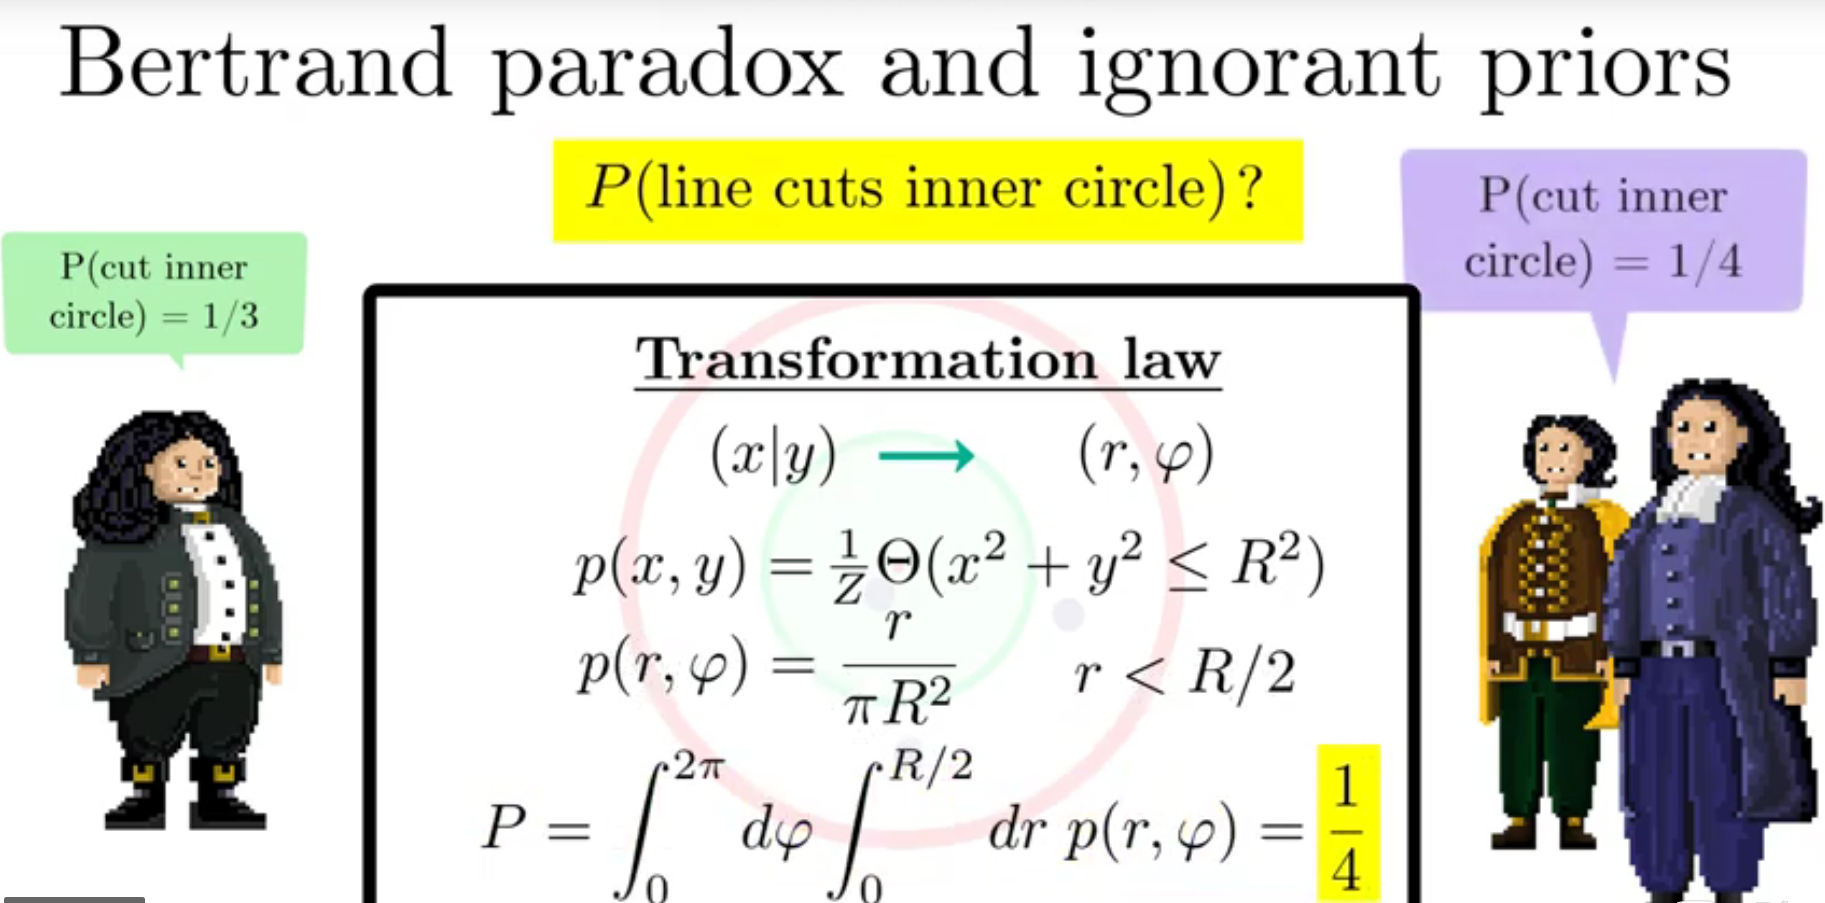
\includegraphics[width=0.75\textwidth]{8_7.png}
\end{figure}
The desired result requires that $r<\frac R2$ and the corresponding probability gives $\frac 14$.

Finally, Laplace suggested to generate the radial distance uniformly between 0 and $R$ resulting in a constant pdf. In that case the probability is $0.5$. 
The question is now, \textit{which algorithm describes the physical experiment?}\\

\fbox{\parbox{\linewidth}{\textbf{Question 6.} Guess who is right! What is the probability for a free day (= that the line does not cut the inner circle)? Do you know why?\\
a) Laplace: It is a 50\% chance to have a free day.\\
b) Pascal: It is a 75\% chance to have a free day.\\
c) Bernoulli: It is a 67\% chance to have a free day.
}}
\\

This question is already on the mind of scientists for generations and still is.
We can phrase this problem more generally: If we know nothing about the
pdf apart from the definition of the setup - so there are no experimental
data or additional theoretical constraints - what is the correct way to find an
un-informative prior? So how do we assign probabilities in the continuous way?
Such an object is also called an \textbf{ignorant prior}.\\

For ignorant priors Ed Jaynes came up with the following idea. \textit{If there is a
continuous and invertible map $\vec{T}(\vec{x})$ from one set of variables $\vec{x}$ to a
new set $\vec{y}$, then the corresponding pdfs should be the same, i.e $p(\vec{y})=p(\vec{x})$.} In the case of the die it
means that putting the pips on different sites of the cube should not modify the probability mass function.
In other words, \textit{the probability mass function should be invariant against
permuting the indices}, which results in the well-known uniform distribution.
Since the mapping in the continuous case is assumed to be continuous as
well, we can introduce a parameter$\epsilon$ such that for $\epsilon\rightarrow 0$ the mapping is the
identity. \[\lim_{\epsilon\rightarrow 0}\vec{T}_{\epsilon}(\vec{x})=\vec{x}\]

Using the transformation law from above and the invariance properties of
the pdf, Jaynes came up with the following equation for the pdf:%8_8
 \begin{figure}[H]
	\centering
	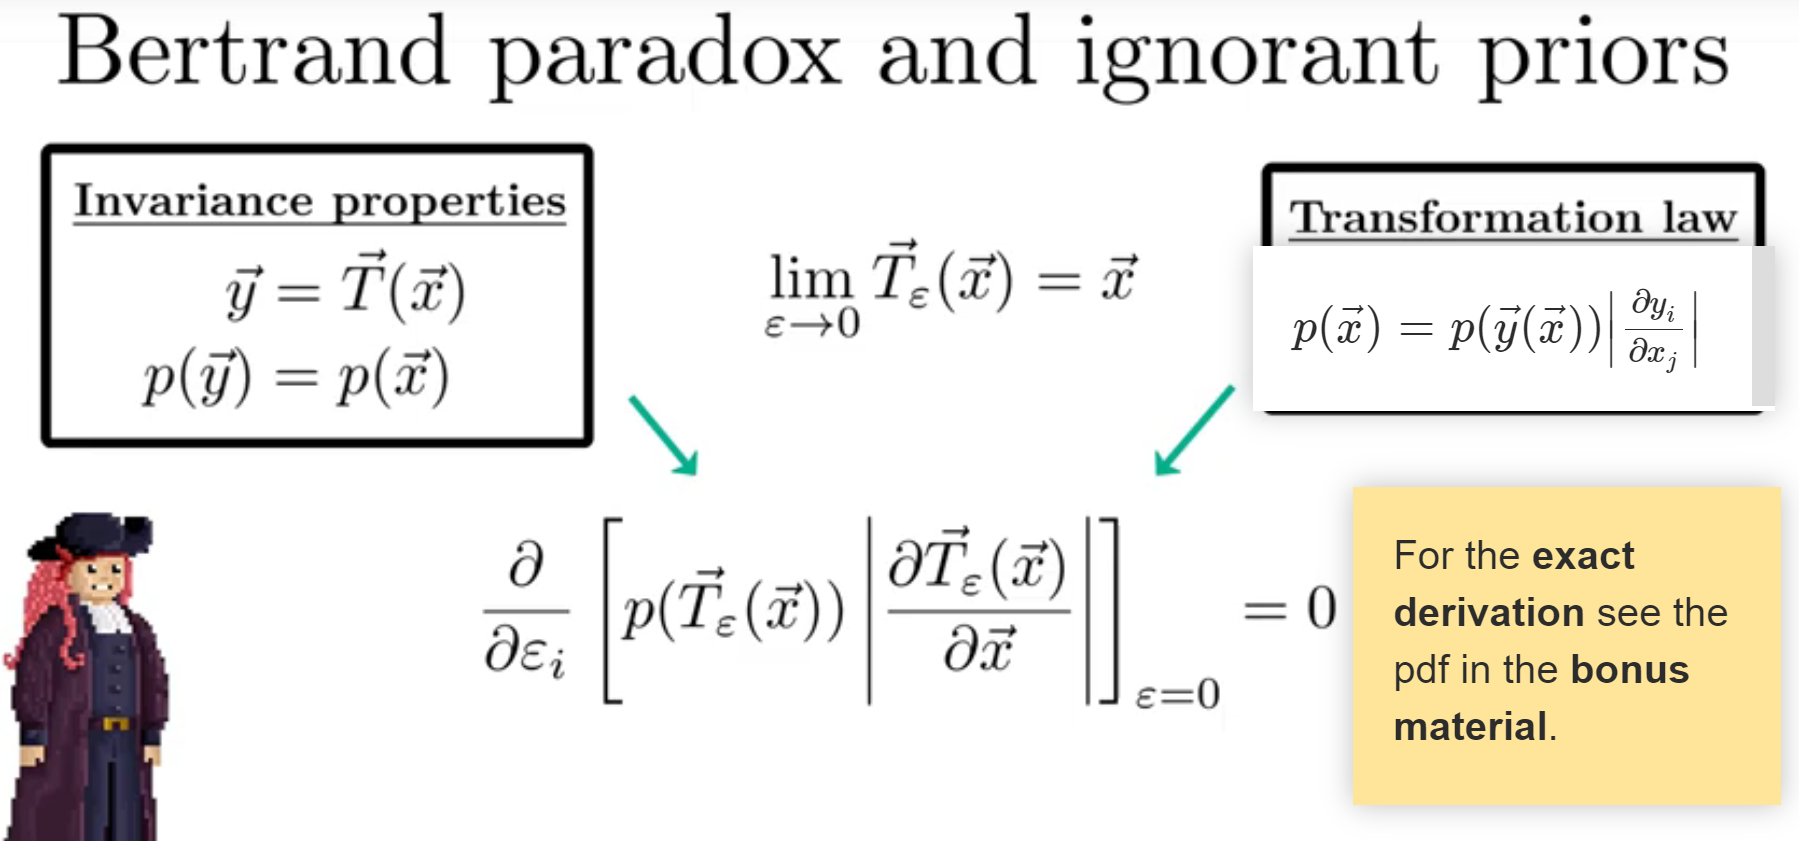
\includegraphics[width=0.75\textwidth]{8_8.png}
\end{figure}

Let’s illustrate this approach for a \textbf{scale variable} $y=\alpha x$. A scale variable $x$ is a
\textit{non-negative quantity for which the pdf should be scale invariant}. In this case, the infinitesimal transformation has the following form:\[T_{\epsilon}=(1+\epsilon)x\]
Jaynes’ equation can be solved by elementary tools
and the result is 
\begin{equation*}\boxed{p(x)=\frac 1x
}\end{equation*}\\
Note that this is a so-called \textbf{improper pdf}, as it \textit{cannot be normalized}. In the
frame of Bayesian probability theory, such a prior is not forbidden as long as
the resulting posterior is normalizable.
This scale-invariant pdf is often called \textbf{Jeffreys’ prior}, although it is only a
special application of Jeffreys’ idea.\\

The uninformative prior pdf of parameters a depends of course on the
meaning of the parameters. In many cases these are uniquely determined
by the likelihood function $p(d|a)$. In that case, a pdf that is invariant against reparameterization is given by $p$ of a is given by the determinant of g (see picture).%8_9
 \begin{figure}[H]
	\centering
	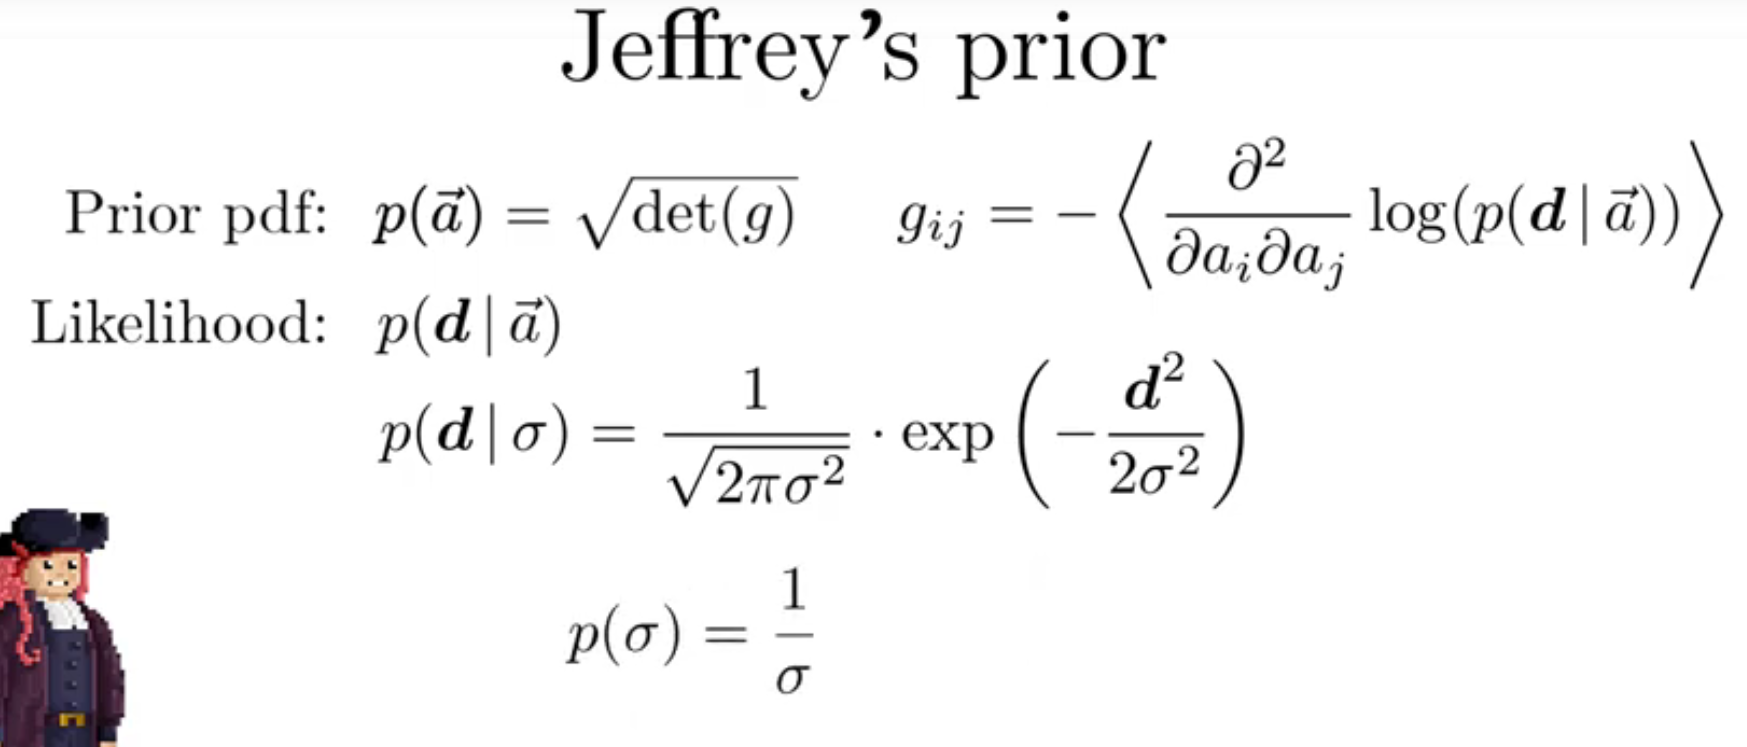
\includegraphics[width=0.75\textwidth]{8_9.png}
\end{figure}

A typical example of the scale variable is the standard deviation $\sigma$ that enters
a Gaussian likelihood. This is a nice and informative exercise for the application of Jeffrey’s prior. The result is the same as that obtained by Jaynes’
approach $p(\sigma)=\frac{1}{\sigma}$\\

Ed Jaynes applied the principle of transformation invariance to the Bertrand paradox.
He used the following transformations under which the problem is invariant:%
\begin{enumerate}
	\item Translation of the center of the circle
	\item Rescaling of the radius
	\item Rotation of the circle about the center
\end{enumerate} 
The solution of his equation yields the same result that Laplace proposed :\\
\[p(r)=\text{const}=\frac 1R\]

There is another way to approach the Bertrand paradox. Since the lines
are drawn randomly and without knowing the position of the circle, we can
equally well draw the line first and then randomly place the circle on the
plane. The circle is uniquely defined by its center and therefore this is equivalent to randomly choosing the coordinates $x$ and $y$ of the center. If we define
the direction of the line as the $x$-axis, then the $x$-coordinate of the center is
irrelevant. Consequently, the distance of the line from the center of the circle is given by the absolute value of $y$. As the coordinates of the center are
chosen at random, the distance is a uniform random variable corroborating
Jaynes' result.\\%

\section*{Maximum Entropy}
We have encountered the \textbf{maximum entropy principle} already in the discrete case. It
was introduced to obtain the probability mass function in the case of testable
information given for instance in the form of mean values. Maximum entropy can also
be invoked for pdfs given testable information for instance in the following form:\[\int \text{d}x f_i(x)p(x)=\mu_i\]

The only complication in the continuous case is that the entropy is not entirely what you would expect.\\
\begin{equation*}\boxed{S(p)=-\int dx p(x)ln\left(\frac{p(x)}{p_0(x)}\right)
}\end{equation*}\\

The function $p_0(x)$ is sometimes called the \textbf{default model}, because the MaxEnt
solution without any constraints apart from normalization yields $p(x)=p_0(x)$.\\
The deeper reason why we have a default model in the continuous case and
not in the discrete case is that the transition by discretization from the
continuous to the discrete case is not unique.
The default model plays the role of an ignorant prior.
Otherwise, the implementation of testable information in the maximum entropy procedure is the same as in the discrete case.
On passing we want to discuss a simple application from statistical physics.
We want to infer the pdf $p(x)$ of particles at the height $x$ above the earth.
The mean potential energy of these particles is proportional to the mean
height.\[E=mg\int x p(x)\text{d}x \propto \langle x\rangle\]

In a canonical ensemble the mean energy is given by $k_BT$
So the constraint has the following form: \[ \langle x \rangle = \int xp(x)\text{d}x = \frac{k_BT}{mg}\]

Maximizing the entropy yields the \textbf{Barometric formula} $P\propto \exp(-\alpha x)$.
Note that $x$ is \textit{not
a scale variable here as there is an upper limit for it}. Therefore, a uniform prior
is adequate, which is corroborated by the experimental observation for free
particles without potential energy.\\

In closing, it should be mentioned that this form of entropy is also called
 \textbf{cross-entropy} or in other context the  \textbf{Kullback-Leibler distance}.
 \[d_{KL}(p,q)=\int_{-\infty}^{+\infty}p(x)log\left(\frac{p(x)}{q(x)}\right)\text{d}x\]
 It can be
considered as distance between distributions $p(x)$ and $p_0(x)$, and it plays
an important role in machine learning.\\

\fbox{\parbox{\linewidth}{\textbf{Question 7.} Which of the following statements is true?\\
a) We need a default model $p_0$ in the entropy $S$ in the continuous case, since the mapping from the continuous to the discrete case is not unique.\\
b) The height variable $x$ when deriving the barometric formula is uniform since the earth has a finite atmosphere.\\
c) We need a default model $p_0$ of the entropy $S$ in the continuous case, since variables are scale invariant.
}}
\\


\section*{The lighthouse problem}
The lighthouse problem that Lyra addressed in the adventure is another
example of the  \textbf{transformation of coordinates}. Let $x_0$ and $y_0$ be the coordinates
of the lighthouse and let the coast line define the $x$-axis with the origin of
the coordinate system being on the coast line.
The lighthouse emits light signals that are uniformly distributed in the rotation angle $\varphi$ about the lighthouse axis. We are interested in the pdf for a
light signal being detected at point $\boldsymbol{x}$ on the coast line.
The following relation exists between the coastline position x and the
angle $\varphi$, and the transformation law yields the desired pdf for $\boldsymbol{x}$ from the uniform pdf for
the angle.\\ %8_10
 \begin{figure}[H]
	\centering
	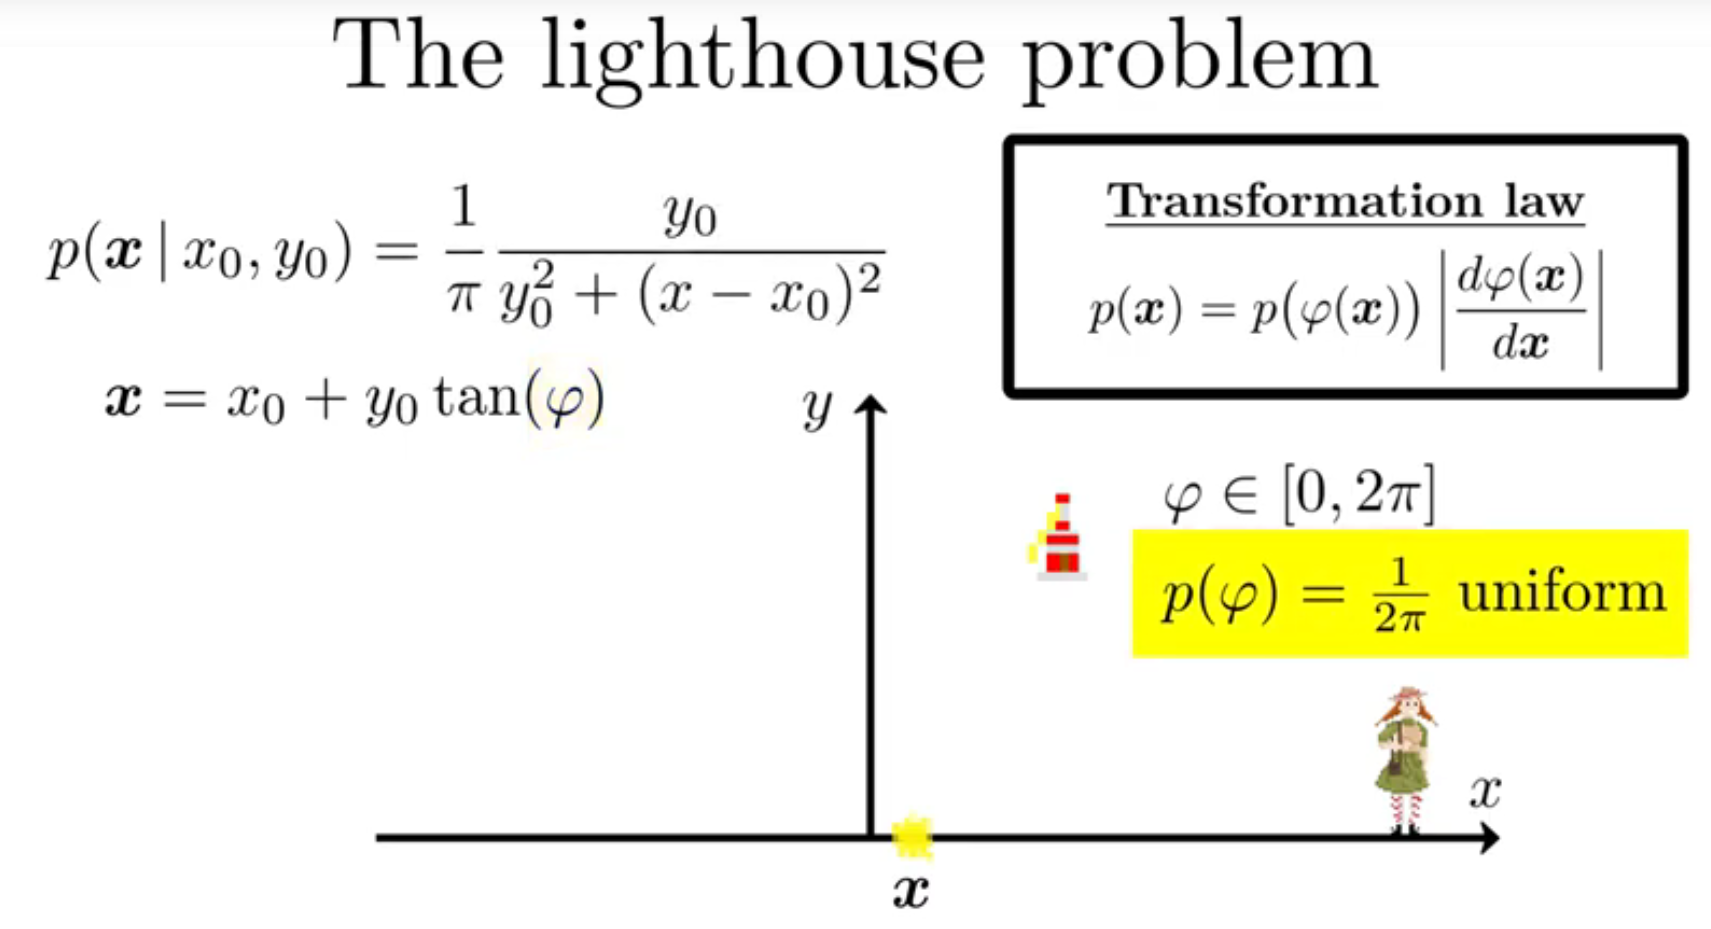
\includegraphics[width=0.75\textwidth]{8_10.png}
\end{figure}

$p(\boldsymbol{x}|x_0,y_0)$ is the probability to find a light signal at position $\boldsymbol{x}$ given the parameters
$x_0,y_0$ and therefore it represents the likelihood of the problem.
We assume for simplicity that the data points $\boldsymbol{x}_i$ are uncorrelated. Bayes
theorem then yields for the desired pdf for the position of the lighthouse the following form.
\[p(x_0,y_0|\boldsymbol{x})=\frac 1Z \prod_i p(\boldsymbol{x}_i|x_0,y_0)p(x_0,y_0)\]
The prior probability depends on our knowledge about lighthouses.
\textit{In the Pluto notebook you can gain experience with this problem and see that
it is indeed possible to locate the lighthouse on the basis of the distribution
of the light flashes on the coastline.}

\section*{Important distributions}
There are many important distributions for continuous variables. Here we
only want to mention the most popular ones.
We have repeatedly used Bayes’ theorem to compute the posterior pdf for a
parameter a given some data d.
Let’s first ignore the prior $p(a)$, then the posterior is proportional to the likelihood $p(a|\boldsymbol{d})\propto p(\boldsymbol{d}|a)$.
In case of a counting experiment with a Poisson likelihood the parameter
$a$ corresponds to the mean $\mu$ and the data are the counts $\boldsymbol{N}$. Then the
posterior is of the following form:
\begin{equation*}\boxed{p(\mu|\boldsymbol{N})\propto e^{-\mu}\mu^\boldsymbol{N}
}\end{equation*}\\
This function is a  \textbf{Gamma-distribution}, that is defined for the range $x\in [0,\infty)$
and with the correct normalization it reads.%8_11
 \begin{figure}[H]
	\centering
	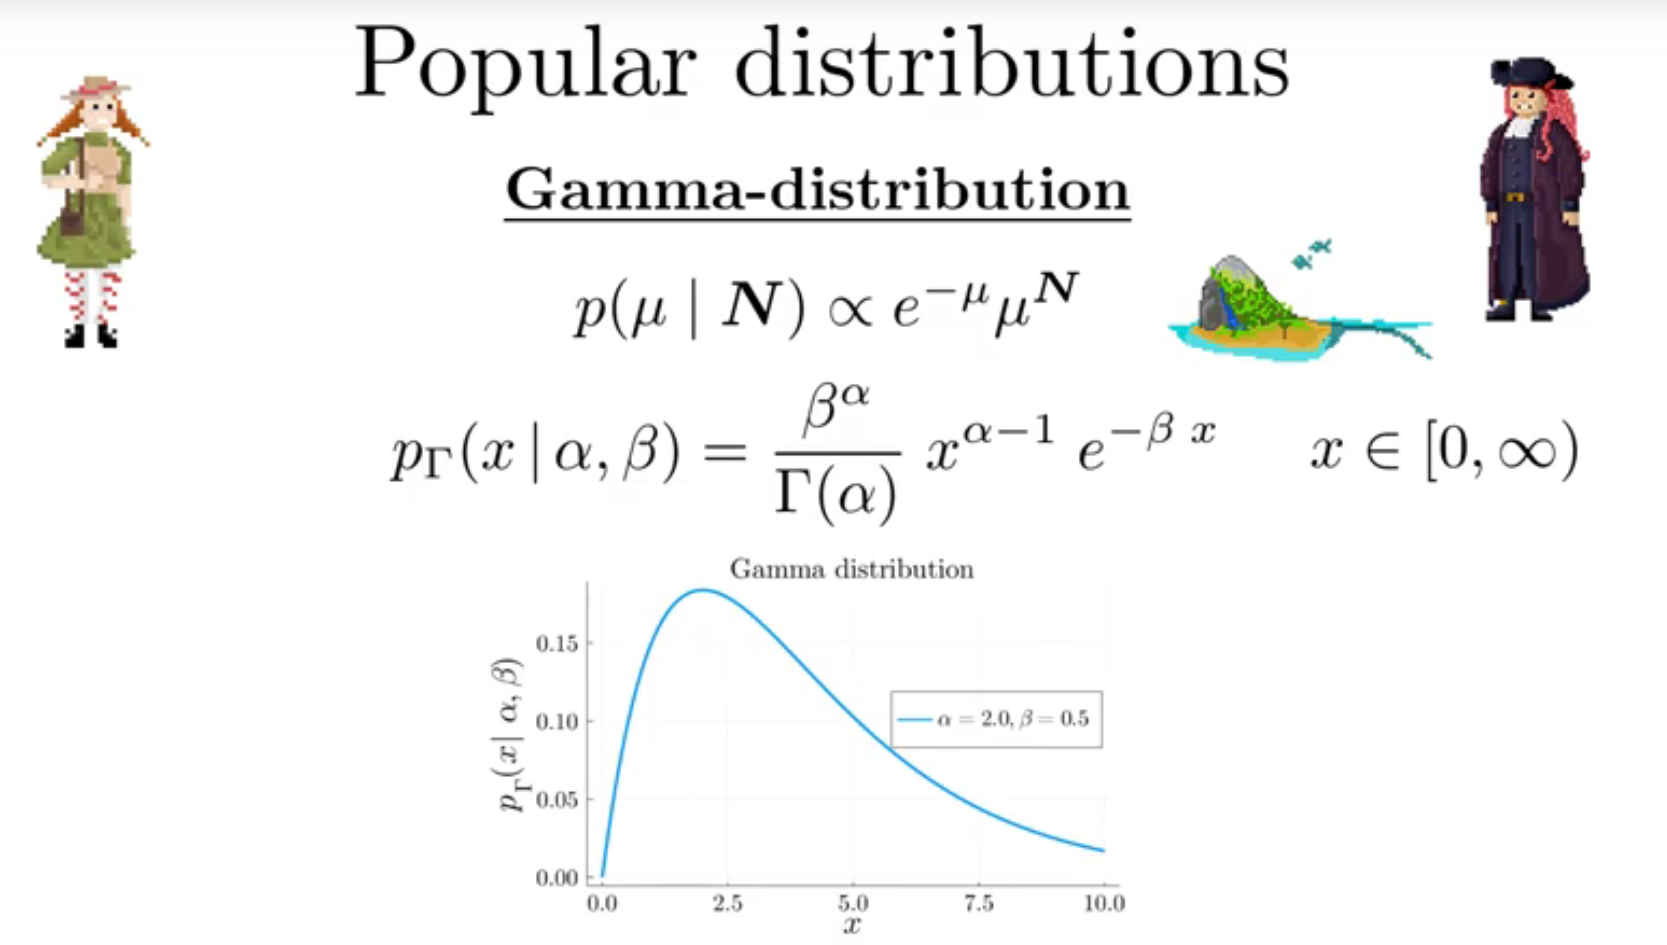
\includegraphics[width=0.75\textwidth]{8_11.png}
\end{figure}
It has a \textit{power-law dependence for small x} and \textit{decays exponentially for large
x}. Mean and variance are given by the following expressions.
\begin{equation*}\boxed{\langle x\rangle = \frac{\alpha}{\beta} \qquad \text{var}(x)=\frac{\alpha}{\beta^2}
}\end{equation*}\\
They can easily be derived from the Gamma function which is part of
the normalization.
\[\Gamma(\alpha):=\int_0^{\infty}t^{\alpha-1}e^{-t}\text{d}t\]
The Gamma function has a very convenient recursion relation
and for an integer argument it is related to the factorial: \[\Gamma(N)=(N-1)! \quad N\in\mathbb{N}\]

Moreover, we want to mention that $\Gamma(\frac 12)=\sqrt{\pi}$.
Special cases of the Gamma distribution are the  $\mathbf{\chi^2}=\Gamma(\frac n2, \frac 12)$ \textbf{distribution} 
and the  \textbf{exponential distribution} $\Gamma(1, \beta)$.\\%

So far we have only discussed the likelihood which lead to the Gamma distribution. If we include an arbitrary prior, then the posterior will be different.
For that reason it is common practice to also use a Gamma distribution for
the prior. This is not a significant restriction, as prior knowledge is typically
vague and the Gamma distribution is very flexible and can cover a wide range
of prior knowledge. Such a so-called  \textbf{conjugate prior} has the advantage that
the posterior is still a Gamma distribution and mean and covariance can be
computed analytically.\\


Now we turn to a Bernoulli experiment with sample size $N$. Here, the parameter a
corresponds to the intrinsic probability $q$ and the data is the number $K$ of
occurrences of the outcome of interest, so $p(a|d)=p(q|K,N)$. Then the posterior is of the following form:
\begin{equation*}\boxed{p(q|K,N))\propto q^K(1-q)^{N-K}
}\end{equation*}\\
This function is a  \textbf{Beta-distribution}, which has the range$x\in [0,1]$ and the
normalized distribution reads.%8_12
 \begin{figure}[H]
	\centering
	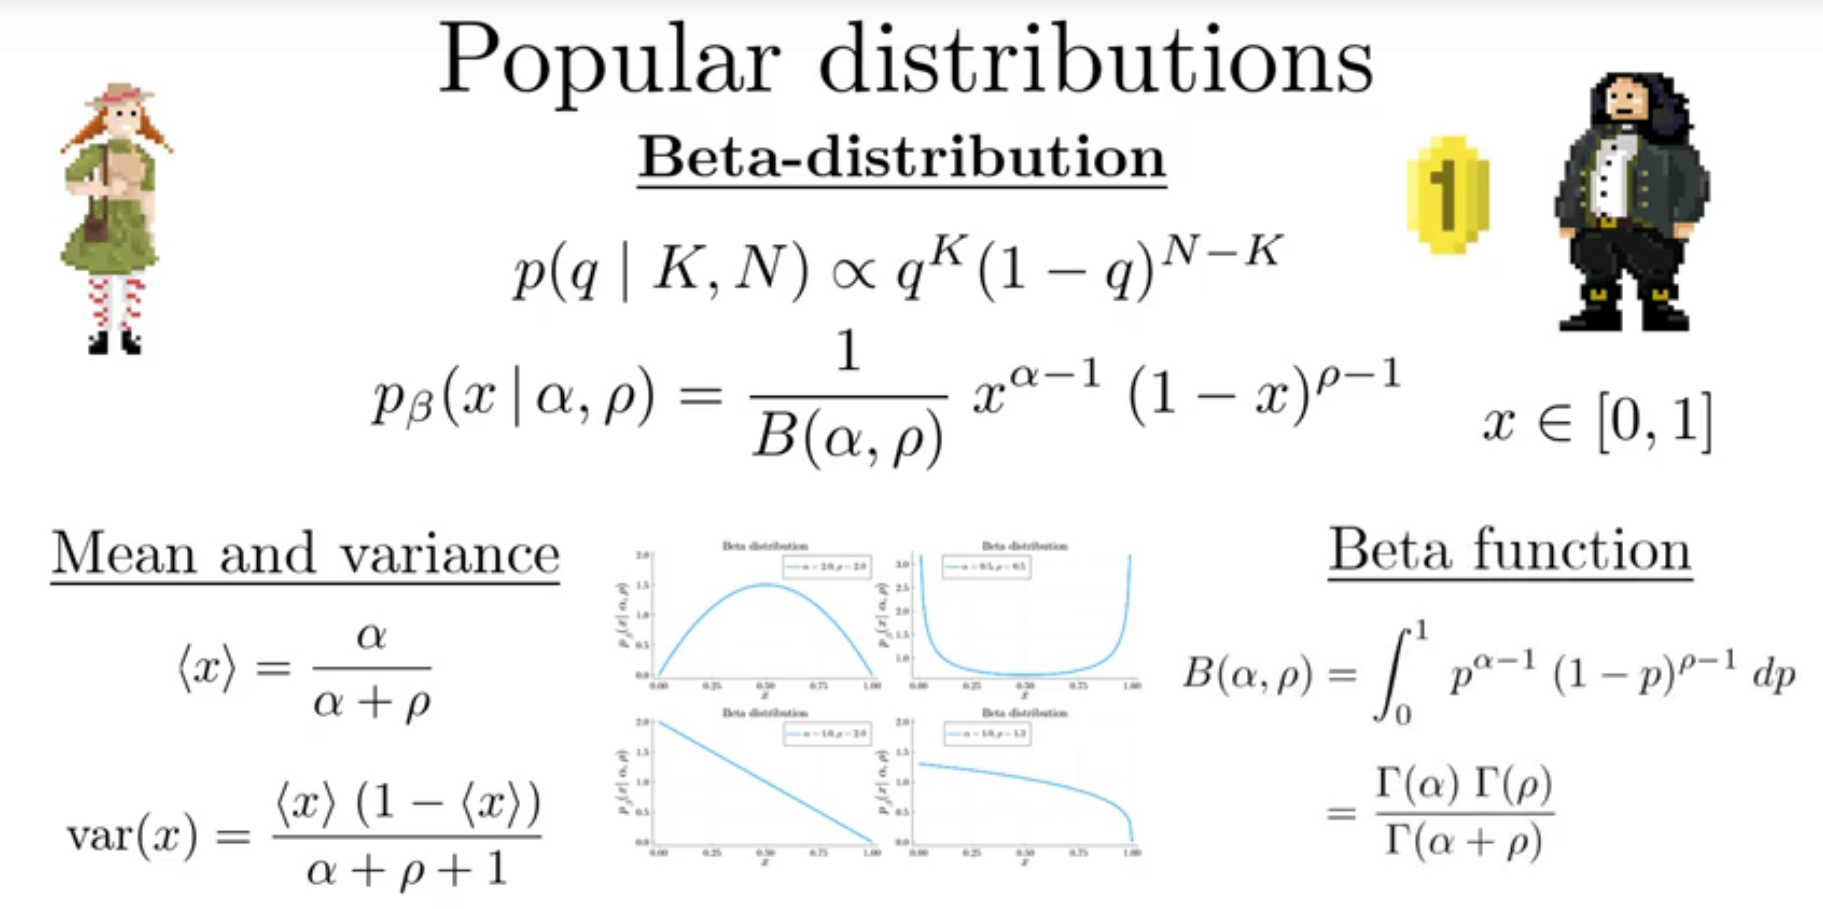
\includegraphics[width=0.75\textwidth]{8_12.png}
\end{figure}
Mean and variance
can be determined by means of the beta function.
It also enters the normalization of the beta distribution.
In case of a Bernoulli experiment the conjugate prior is therefore a Beta
distribution.\\

Finally, we want to mention the  \textbf{Gaussian distribution}, which we have already
encountered several times. The Gaussian is of central importance for the
description of experimental noise and the range of the random variable in
the one-dimensional case is the entire real axis. The normalized Gaussian has a mean and a variance which is given by the following expressions.\\%8_13
 \begin{figure}[H]
	\centering
	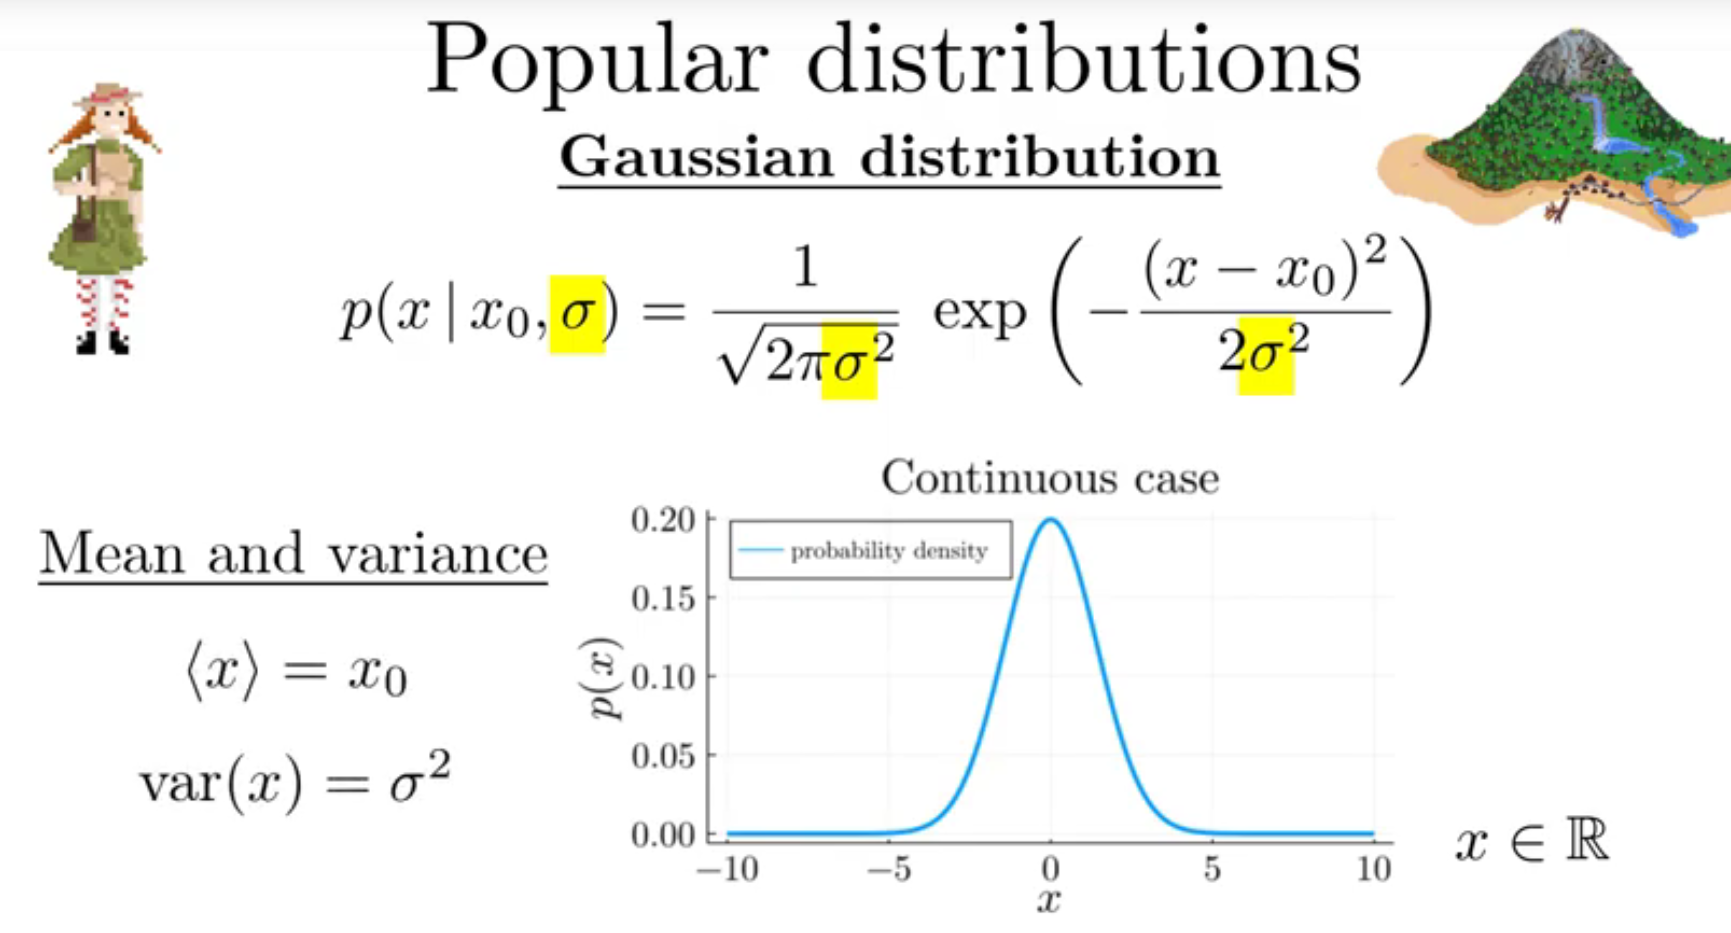
\includegraphics[width=0.75\textwidth]{8_13.png}
\end{figure}
\textit{See the Pluto notebook about popular distributions and study the possible
shapes that emerge by varying the parameters.}\\

\fbox{\parbox{\linewidth}{\textbf{Question 8.} Match the distributions: \{Gauss, Gamma, Beta\}\\
The domain of the .............. distribution is $x\in[0,1]$, as it describes the probability of a probability.\\
The ......... distribution is the conjugate prior of a Poisson Likelihood.\\
The .......... distribution is parametrized by mean and variance.
}}
\\

\section*{Benford's law}
Lyra in the adventure also mentioned a very interesting discovery that \textit{the
leading digits of large numbers form a pattern} no matter what is considered: %8_14
 \begin{figure}[H]
	\centering
	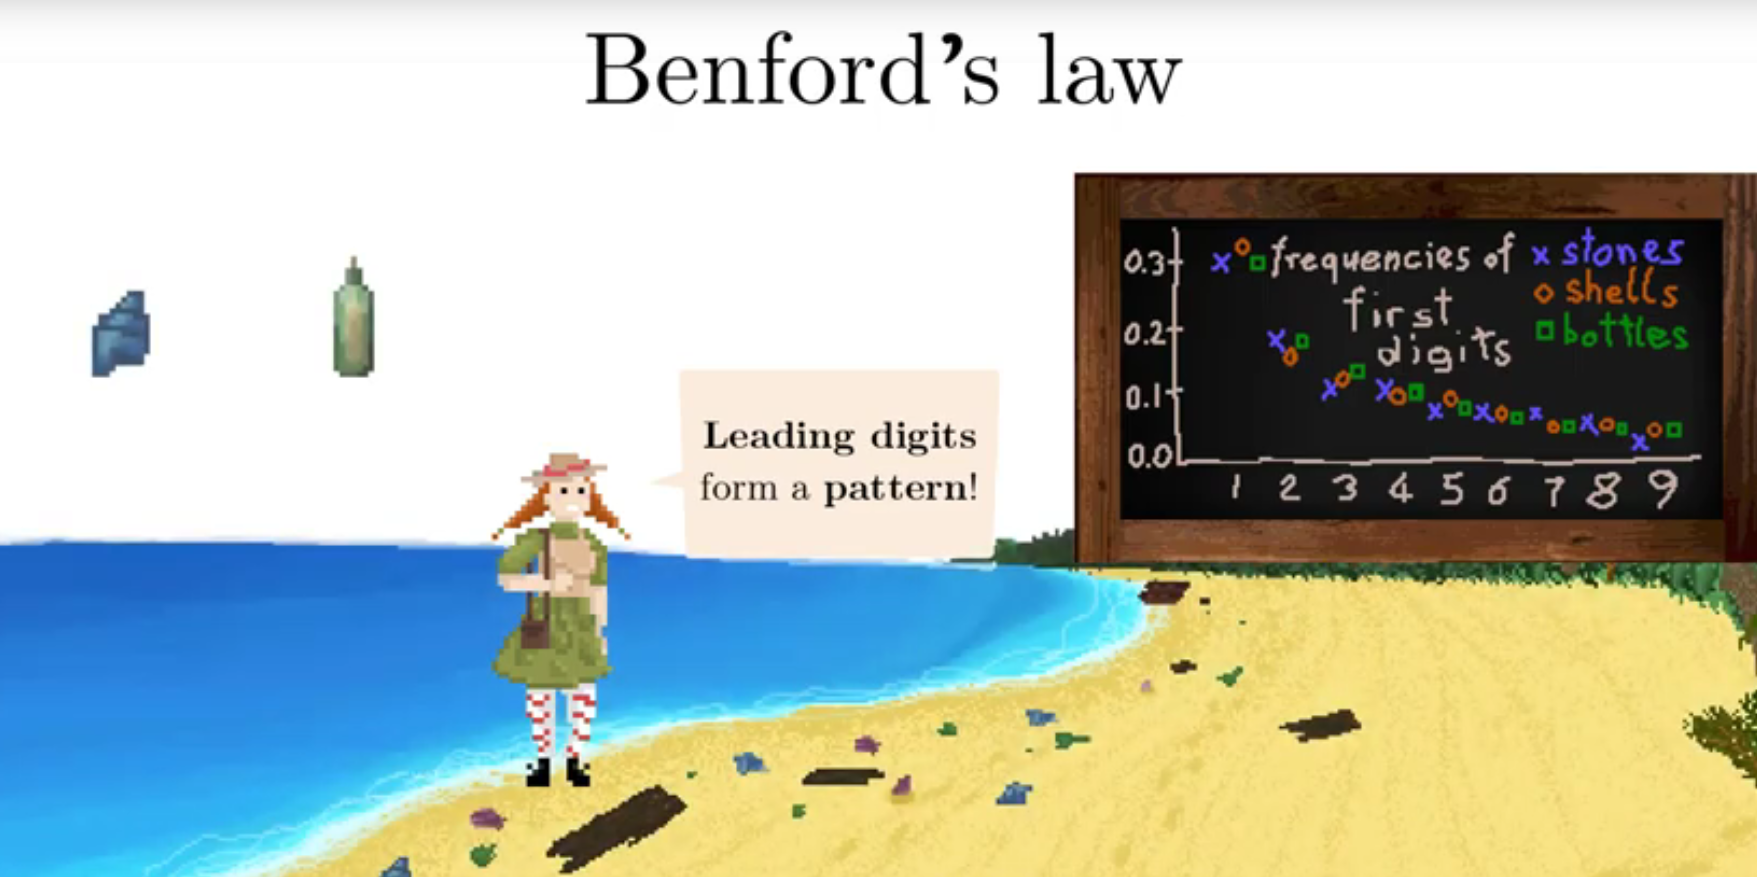
\includegraphics[width=0.75\textwidth]{8_14.png}
\end{figure}
For the amount of collected shells, bottles, coloured stones per day, the leading numbers all behave the same and
they are  \textbf{not} uniformly distributed. This is in contradiction to the principle
of indifference.\\
This phenomenon has to do with  \textbf{scale invariances}. We have seen before that
the pdf of scale invariant quantities $x$ is given by Jeffrey’s prior $p(x)\propto \frac 12$.
Put differently the pdf for log($x$) is uniform, so for $y=\log_{10}(x)\rightarrow p(y)= \text{const}$.
If you recall the intervals on logarithmic axes you may have noticed that the
interval sizes \textit{decrease} from 1 to 9. %
Let’s consider numbers x between 1 and 9.99999$\ldots$

The leading digit corresponds to the interval $x \in [1,2)$.
Then the probability is $P_1\propto \int_1^2\frac{\text{d}x}{x}\ln(2)-\ln(1)$.
In general, the probability that the leading digit has the value $I$ is proportional to $\log(I+1)-\log(I)$.
With the correct normalization for all possible digits 1 up to 9 we have the probability that the leading digit is $I$ given by $\log_{10}(I+1)-\log_{10}(I)$
This distribution is depicted in the figure.\\%8_15
 \begin{figure}[H]
	\centering
	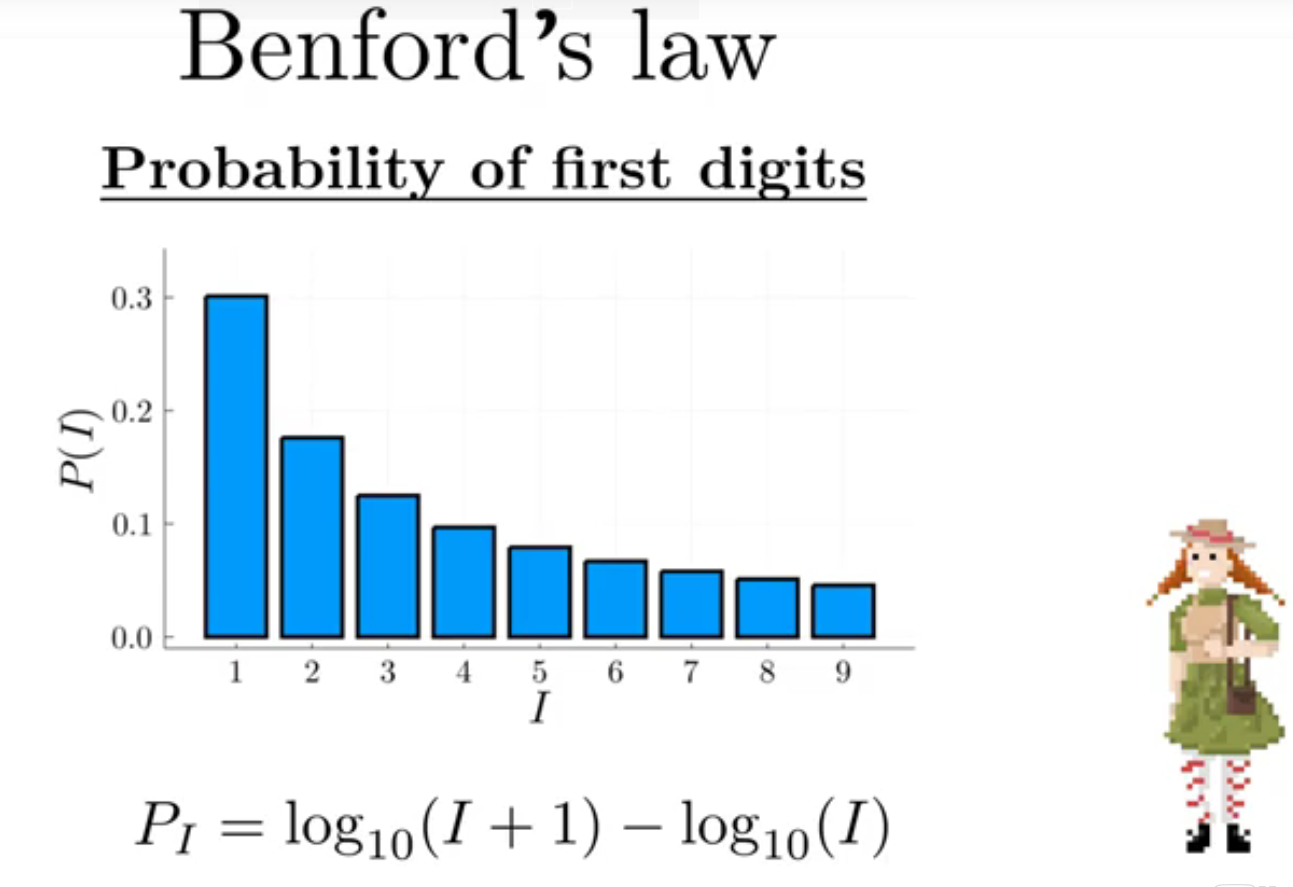
\includegraphics[width=0.75\textwidth]{8_15.png}
\end{figure}

The same result is obtained if the numbers are in the interval 10 to 99.9999
or a 100 to 999.999 and so on.
Actually, the same law holds true also for \textit{counting experiments when the
numbers vary over many orders of magnitude}. Also in this case the probability mass function is \textit{uniform on a logarithmic scale} or  \textbf{log-uniform} as it is
sometimes called.\\

\fbox{\parbox{\linewidth}{\textbf{Question 9.} Which of the following variables could be scale invariant?\\
a) Rain drops per day/km$^2$\\
b) The results of repeated dice throws, using a 100 faced die\\
c) The number of sand grains in your shoes
}}
\\

\textit{You will find a Pluto notebook to perform random experiments with log-uniform distributions.}\\


This concludes lesson 8. We have learned about continuous variables and
how to assign prior probabilities using the principle of transformation invariance or the maximum entropy principle. We have discussed Bertrand's paradox and know now why Benford’s law
describes the leading digit of counting lists and measurement tables.
Check out the interactive Pluto notebooks to solve the lighthouse problem,
to do your own Benford computer experiments, and to experiment with
various popular distributions. Feel free to ask questions in the forum and feel encouraged to test your knowledge in the quiz.

\vspace{2cm}
\begin{minipage}[t]{1\textwidth}
	\raggedleft
	\centering
	
\includegraphics[width = 0.20\textwidth]{CC-BY_icon}
	\vspace{0.2cm}
	
	\centering
	{\large ITPCP, TU Graz} \\
	https://creativecommons.org/licenses/by/4.0/legalcode
\end{minipage}
\end{document}